\chapter{Technical Background}
\label{chapter:background}

This chapter introduces the concepts needed to understand the design and
evaluation of the project. It begins with phishing and URL structure, then
explains URL representations, the classifier families used in the experiments,
and the role of generative adversarial networks. The final sections explain why
data quality, distribution shift, class balance, thresholds, and complete
evaluation metrics are essential when judging a phishing detector.

\section{Phishing and URL-Based Detection}

Phishing is an attempt to impersonate a trusted person or service so that a user
performs an unsafe action. The action may be entering credentials, sending a
payment, opening a file, or visiting a malicious webpage. A phishing campaign
usually combines a delivery method, a deceptive message, a destination URL, and
a page designed to appear trustworthy. The URL is therefore only one part of an
attack, but it is available early enough to support a warning before the user
interacts with the destination.

Software-based phishing detection includes blacklists and whitelists, heuristic
rules, webpage-content analysis, visual comparison, network or domain evidence,
and machine-learning models. Blacklists are effective for threats that have
already been reported, but they cannot contain every newly created or rapidly
changed address. Content and visual approaches can provide more evidence, but
they require the page to be fetched and may introduce delay or risk. A URL-only
model uses the address that is already available to the browser and can run
without downloading the full page \citep{alahmadi2022pdgan,alalyan2020robust}.

This project uses URL-only classification as the primary detector. This choice
supports fast local inference and makes the experiments reproducible. However,
the model cannot confirm page content, ownership, or later changes. Its output
is a risk estimate based on URL patterns, not proof that a website is malicious.

\section{Structure of a URL}

A Uniform Resource Locator identifies a resource and describes how it can be
accessed. A simplified URL can contain a scheme, host, optional port, path,
query, and fragment. Figure~\ref{fig:url-anatomy} shows these components in an
example address.

\begin{figure}[htbp]
\centering
\footnotesize
\fbox{\parbox{0.91\textwidth}{
\centering
\texttt{https://accounts.example.com/login?session=271\#confirm}\\[0.25cm]
\begin{tabular}{@{}llllll@{}}
scheme & host & port & path & query & fragment \\
\texttt{https} & \texttt{accounts.example.com} & --- &
\texttt{/login} & \texttt{session=271} & \texttt{confirm}
\end{tabular}}}
\caption{Main components of a URL.}
\label{fig:url-anatomy}
\end{figure}

The host itself is hierarchical. In \texttt{accounts.example.com},
\texttt{com} is the top-level domain, \texttt{example} is the registered-domain
label, and \texttt{accounts} is a subdomain. Attackers can place a trusted word
in a subdomain or path even when the registered domain is unrelated to the
service being imitated. Other suspicious patterns can include an IP address in
place of a host name, many nested subdomains, misleading brand tokens, character
substitutions, encoded text, unusually deep paths, or a long query string.

None of these patterns proves phishing by itself. Legitimate authentication,
advertising, cloud storage, redirection, and tracking services may also produce
long and complicated URLs. This is one reason fixed rules often create false
positives. Kan and Nguyen Thi showed that URL components, their lengths,
orthographic patterns, and token order all contain useful classification
information \citep{kan2005fast}. The detector should learn combinations of
evidence rather than treating one feature, such as length, as a final decision.

\section{Representing URLs for Machine Learning}

A learning algorithm requires a numerical representation. This project uses
two complementary representations: manually calculated lexical features and a
character sequence learned by a neural network.

\subsection{Lexical Features}

Lexical features describe measurable properties of the URL string without
visiting the website. Examples include total length, hostname length, numbers of
digits, letters, dots and special characters, digit-to-character ratios,
subdomain count, path depth, query parameters, and the presence of an IP-style
host. Table~\ref{tab:background-feature-groups} groups the main types.

\begin{table}[htbp]
\centering
\caption{Groups of lexical URL features used in phishing detection.}
\label{tab:background-feature-groups}
\small
\begin{tabular}{@{}p{0.22\textwidth}p{0.30\textwidth}p{0.37\textwidth}@{}}
\toprule
Feature group & Examples & Information represented \\
\midrule
Length & URL, host, path, and query length & Overall complexity and unusually long components. \\
Character counts & Dots, hyphens, digits, symbols, and repeated characters & Surface patterns and possible obfuscation. \\
Ratios & Digit, letter, and special-character ratios & Composition independent of absolute length. \\
Host structure & Subdomains, IP-style host, top-level-domain form & How the destination host is organised. \\
Path and query & Path depth, parameters, delimiters, and encoded characters & Structure after the host and possible redirection or tracking. \\
Token indicators & Login, account, verify, update, secure, and brand-like terms & Words commonly used in service and credential contexts. \\
\bottomrule
\end{tabular}
\end{table}

Lexical features are small, fast, and interpretable. They are suitable for
Random Forest and Support Vector Machine models, and they can be added to a
neural model. Their weakness is that the selected list reflects existing human
knowledge. Wang found that both lexical selection and token/vector
representations can be useful, while ensemble classifiers performed strongly in
the reported comparison \citep{wang2022malicious}. However, an attacker can
change a URL in a way that is not well represented by a fixed feature list.

\subsection{Character-Level Representation}

A character-level model first constructs a vocabulary containing the letters,
digits, punctuation marks, and special symbols retained during preprocessing.
Each character is mapped to an integer. URLs are padded or truncated to a fixed
maximum length so that a batch has a consistent shape. An embedding layer then
maps each integer to a learned dense vector.

This representation keeps local spelling, punctuation, and order information.
It avoids assuming that a URL can be tokenised like an ordinary sentence.
Al-Alyan and Al-Ahmadi used this approach with a CNN and a dataset of more than
two million URLs, showing that a URL-only character model can operate without
predetermined features \citep{alalyan2020robust}. Character models still have a
maximum input length, so truncation must be reported and long URLs require
separate evaluation.

\subsection{Hybrid Representation}

The hybrid representation combines a learned character vector with a lexical
feature vector. Before concatenation, numerical lexical values are scaled using
parameters fitted on training data only. The combined vector is passed through
dense layers to produce a phishing score. The character branch can discover
patterns that were not explicitly programmed, while the lexical branch directly
provides stable measurements such as length and path depth.

The term \emph{hybrid} in this report refers to this combination of character
CNN features and lexical features. It does not mean that the model uses page
content, screenshots, or live network requests. To keep model comparisons fair,
all classifiers use the same stored real URL rows and labels, even though their
representations differ according to the algorithm being tested.

\section{Classifier Families}

The experiments include traditional and neural classifiers so that the effect
of GAN augmentation is not judged using one model family only.

\subsection{Random Forest}

A decision tree repeatedly divides samples using feature conditions. A Random
Forest trains many trees using sampled rows and subsets of features, then
combines their outputs. This reduces the instability of a single tree and works
well with mixed nonlinear lexical relationships. It can also provide feature
importance estimates. Its main limitation in this setting is that it uses the
provided feature vector and does not directly learn the complete order of URL
characters.

\subsection{Support Vector Machine}

A Support Vector Machine finds a decision boundary with a large margin between
classes. Linear SVMs can be effective with scaled lexical or sparse text
features. Kernel variants can represent nonlinear boundaries but may become
expensive on very large datasets. Because feature magnitude influences the
margin, scaling must be learned from training data and reused unchanged during
evaluation and deployment.

\subsection{Convolutional Neural Network}

A one-dimensional CNN moves filters across the embedded character sequence.
Each filter can respond to a local pattern such as a token fragment, delimiter
combination, or suspicious character sequence. Pooling forms a fixed-size
summary and dense layers produce the final score. CNN operations can be
parallelised efficiently on a GPU and are suitable for local URL inference.
The URL-only CNN literature supports this design for both ordinary detection and
GAN discrimination \citep{alalyan2020robust,alahmadi2022pdgan}.

\subsection{RNN and LSTM}

A recurrent neural network processes the sequence in order and passes a hidden
state from one position to the next. This gives it a direct representation of
sequence history, but an ordinary RNN can have difficulty preserving
information over long distances. The Long Short-Term Memory network introduces
gates that control what is stored, updated, and exposed. LSTMs can therefore
model longer dependencies, although their sequential calculation is generally
slower than the parallel operations of a CNN.

\subsection{Hybrid CNN Classifier}

The project hybrid feeds the embedded URL to a character CNN and concatenates
the resulting representation with scaled lexical features. A simplified
calculation is

\begin{equation}
\hat{p}=\sigma\!\left(f_{\mathrm{dense}}
\left([f_{\mathrm{CNN}}(x_{\mathrm{char}}),x_{\mathrm{lex}}]\right)\right),
\end{equation}

where $x_{\mathrm{char}}$ is the encoded character sequence,
$x_{\mathrm{lex}}$ is the lexical feature vector, $[\cdot]$ denotes
concatenation, and $\hat{p}$ is the predicted phishing probability or score.
The hybrid is not automatically superior: its value must be established using
the same training rows and frozen evaluations as the other classifiers.

\section{Generative Adversarial Networks}

\subsection{Basic Adversarial Training}

A GAN contains two networks trained with opposing objectives. The generator
$G$ transforms a random vector $z$ into a synthetic sample. The discriminator
$D$ receives real and generated samples and learns to distinguish them. In the
original formulation, the objective is

\begin{equation}
\min_G \max_D V(D,G)=
\mathbb{E}_{x\sim p_{\mathrm{data}}}[\log D(x)] +
\mathbb{E}_{z\sim p_z}[\log(1-D(G(z)))] .
\end{equation}

During alternating training, the discriminator improves its judgement and the
generator receives a learning signal that rewards more believable output
\citep{goodfellow2014gan}. The desired result is not a copy of the training set,
but new samples that follow useful parts of its distribution.

\begin{figure}[htbp]
    \centering
    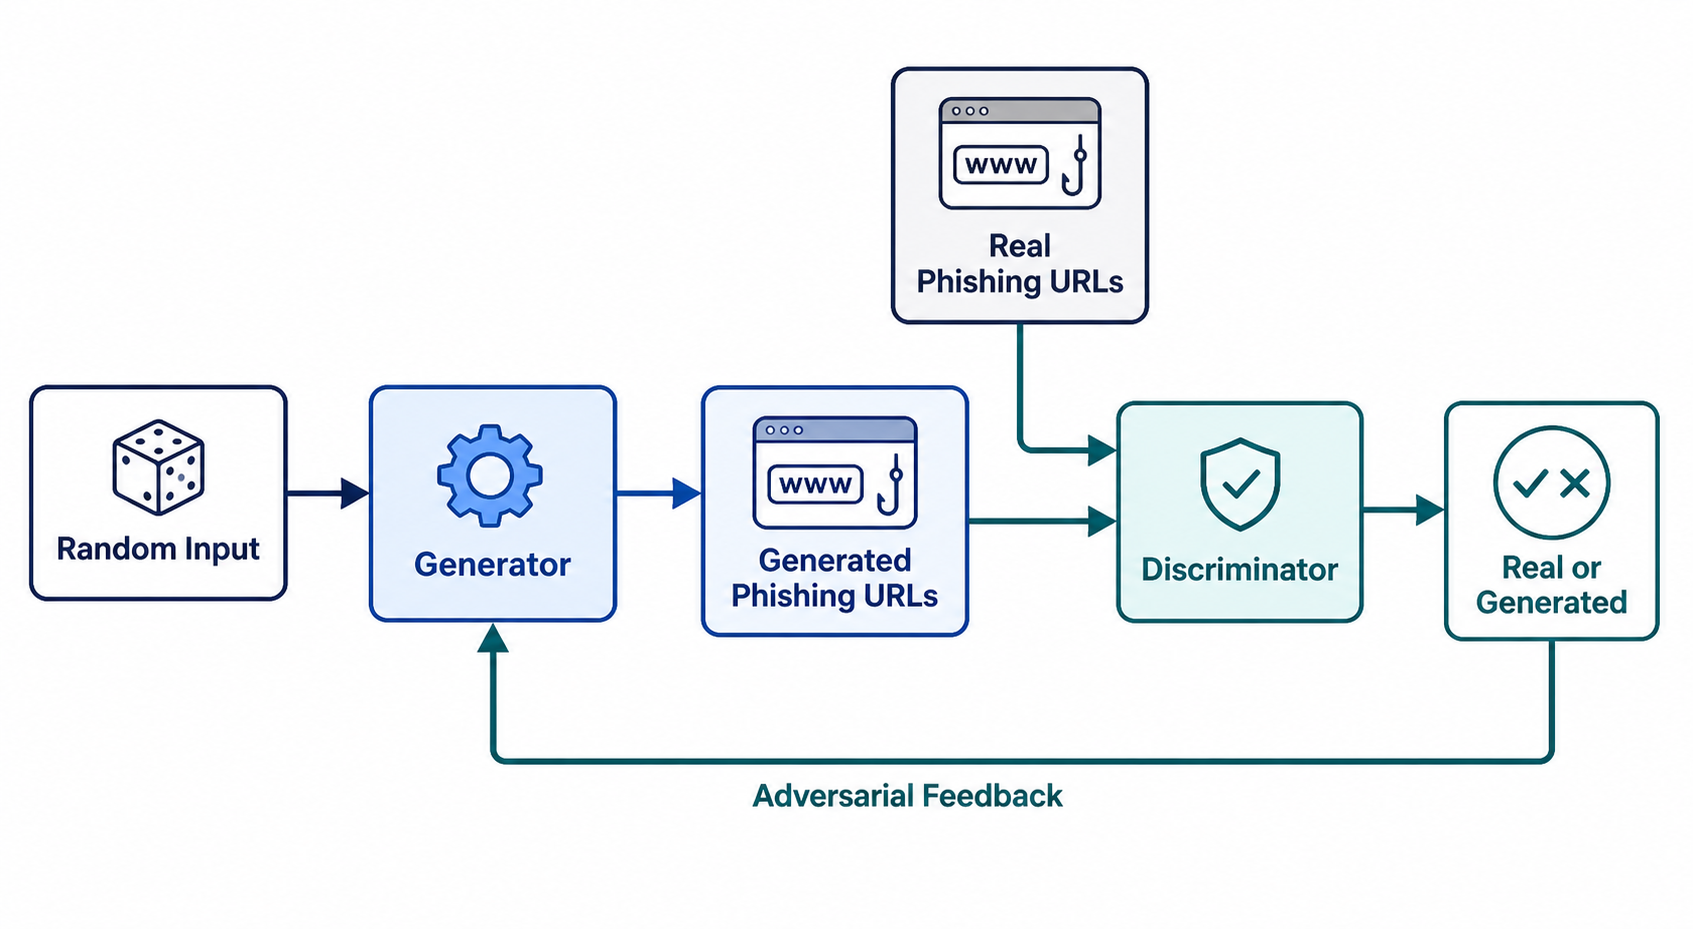
\includegraphics[width=0.92\textwidth]{figures/gan_training_cycle.png}
    \caption{Basic adversarial training cycle adapted to phishing URL generation.}
    \label{fig:background-gan-cycle}
\end{figure}

GAN training can be unstable. If the discriminator becomes too strong, the
generator may receive little useful gradient. If the generator learns only a
small number of successful patterns, it may produce many similar samples; this
is called mode collapse. Loss values alone are therefore insufficient evidence
that generated URLs are useful.

\subsection{Why URL Text Is Difficult to Generate}

Image generators output continuous pixel values, while a URL generator must
select discrete characters. Sampling a character breaks ordinary
back-propagation because the discrete choice is not differentiable. A sequence
generator must also learn syntax: a string may resemble phishing text but still
be unusable if its scheme, host, delimiters, or top-level-domain structure is
invalid.

The Gumbel--Softmax relaxation approximates a categorical choice using a
continuous differentiable vector during training \citep{jang2017gumbel}. As the
temperature is reduced, its output becomes closer to a one-hot character
selection. This provides an end-to-end gradient while retaining discrete
characters when URLs are finally sampled.

SeqGAN takes a different approach and treats sequence generation as a policy.
The discriminator supplies a reward, and Monte Carlo rollouts estimate the
value of incomplete sequences before the final character is produced
\citep{yu2017seqgan}. This can connect a final realism judgement to earlier
character choices, but policy-gradient training may have high variance and is
more complex than ordinary supervised sequence learning.

\subsection{GAN Designs Relevant to the Project}

Several supplied studies motivate the GAN designs considered in this project.
PDGAN uses an LSTM generator to produce phishing URL sequences and a CNN
discriminator to judge URLs \citep{alahmadi2022pdgan}. This pairing is
appropriate because the generator models ordered text while the discriminator
extracts local patterns efficiently. The semi-supervised conditional approach
of Kamran et al. conditions generation on URL and class information and gives
the discriminator both real-versus-generated and benign-versus-malicious tasks
\citep{kamran2022conditional}.

Wasserstein GAN training replaces the original discriminator interpretation
with a critic whose score estimates a distance between real and generated
distributions. WGAN-GP adds a gradient penalty to enforce the required smoothness
without simple weight clipping \citep{gulrajani2017wgangp}. This often improves
training stability, but stable losses do not guarantee syntactically valid or
diverse URLs.

The comparative phishing-GAN study supplied for this project evaluates basic
GAN, DCGAN, WGAN, and SeqGAN models. It reports that generator quality and
discriminator classification do not necessarily rank models in the same order,
and evaluates generated URLs using structural and classifier-challenge evidence
\citep{pham2023evaluation}. This directly supports the decision to measure GAN
quality separately from downstream classifier accuracy.

\section{GAN Augmentation for Defensive Training}

In this project, a generator is trained only on phishing URLs belonging to the
training split. Accepted synthetic phishing URLs are then added to the original
real training rows. Validation, calibration, internal test, and external test
sets remain real and unchanged. If $N_r$ is the number of real training samples
and $N_g$ is the number of accepted generated samples, the generated share of
the resulting training set is

\begin{equation}
r_g=\frac{N_g}{N_r+N_g}.
\end{equation}

This definition is important because ``10\% augmentation'' can otherwise mean
either ten generated samples per hundred real samples or ten generated samples
per hundred total samples. The report states the exact counts for each
experiment.

Generated data can help if it adds realistic patterns that are missing or rare
in the available phishing data. It can hurt if it contains invalid syntax,
repeated templates, generator artifacts, incorrect labels, or structures that
do not match real phishing URLs. More synthetic data is therefore not assumed
to be better. A decrease in accuracy or F1-score is a valid result and should
not be hidden by changing the augmentation percentage after viewing the test
set.

\section{Evaluating Generated URL Quality}

Classifier performance alone cannot show what a GAN learned. The generated
pool is evaluated before augmentation using the following checks:

\begin{description}
\item[Validity:] whether the candidate can be parsed and contains an acceptable
host and URL-like structure;

\item[Uniqueness:] the percentage of generated candidates remaining after exact
duplicates are removed;

\item[Novelty:] whether a generated URL is absent from the real training,
validation, and test data;

\item[Structural realism:] whether length, components, delimiters, top-level
domain form, and lexical statistics fall within plausible real-data ranges;

\item[Diversity:] whether candidates cover different lengths, tokens, hosts,
paths, generators, and clusters rather than one repeated template; and

\item[Classifier challenge:] whether frozen real-only classifiers find the
candidate difficult or place it near their decision boundaries.
\end{description}

A challenging sample is not automatically realistic. A malformed artifact may
confuse a classifier precisely because it is outside both real classes.
Realism, novelty, and challenge must therefore be considered together. The
selection rule must also be frozen before final test evaluation so test labels
cannot influence which generated samples are accepted.

\section{Distribution Shift and Data Leakage}

\subsection{Distribution Shift}

Training and test data are identically distributed only under an idealised
assumption. In practice, legitimate URLs from top-domain lists differ from URLs
observed during normal browsing, and phishing feeds differ in verification
rules, collection time, campaign types, and URL lifetime. These differences are
called distribution shift. A model may learn the source rather than the class;
for example, protocol style or URL length can accidentally identify which feed
supplied a sample.

The large URL-only CNN study warns that models should be kept current and notes
sampling problems caused by representing legitimate data using only highly
ranked sites \citep{alalyan2020robust}. For this reason, this project uses both
internal and identity-disjoint external evaluations, including realistic
low-phishing scenarios and long legitimate URLs. Strong internal accuracy is
not treated as proof of deployment readiness.

GAN augmentation does not predict a future zero-day pattern. It recombines
patterns learned from available phishing training data. It may improve coverage
of nearby variations and make a classifier less dependent on a few templates,
but it cannot guarantee knowledge of a genuinely new attacker behaviour.

\subsection{Data Leakage}

Leakage occurs when information from validation or test data affects training.
Examples include duplicate URLs across splits, the same domain identity in
training and test sets, fitting a scaler on all rows, selecting a threshold on
the final test, or filtering generated samples using final test performance.
Leakage produces optimistic measurements that may disappear in real use.

The controlled pipeline therefore deduplicates and checks overlaps, fits
preprocessing on training data, trains GANs on training phishing URLs only,
selects thresholds on separate development data, and keeps final evaluation
sets frozen.

\section{Evaluation Metrics}

For the positive class ``phishing'', a true positive (TP) is a phishing URL
correctly detected; a false positive (FP) is a legitimate URL incorrectly
flagged; a true negative (TN) is a legitimate URL correctly accepted; and a
false negative (FN) is a phishing URL missed by the detector.

\begin{align}
\mathrm{Accuracy} &= \frac{TP+TN}{TP+TN+FP+FN},\\
\mathrm{Precision} &= \frac{TP}{TP+FP},\\
\mathrm{Recall} &= \frac{TP}{TP+FN},\\
\mathrm{F1} &= 2\frac{\mathrm{Precision}\cdot\mathrm{Recall}}
{\mathrm{Precision}+\mathrm{Recall}},\\
\mathrm{FPR} &= \frac{FP}{FP+TN},\\
\mathrm{FNR} &= \frac{FN}{FN+TP}=1-\mathrm{Recall}.
\end{align}

Accuracy can look high in a deployment-like dataset where phishing is rare,
even if many phishing URLs are missed. Precision indicates how many phishing
warnings are correct and is strongly affected by class prevalence. Recall and
FNR measure missed attacks, while FPR measures disruption to legitimate
browsing. F1 balances precision and recall but does not include true negatives.

ROC-AUC evaluates how well scores rank positive examples above negative ones
across thresholds. It is useful for model comparison, but it does not select an
operating threshold or directly describe warning precision in a low-phishing
environment. This project consequently reports the complete metric set and the
confusion counts rather than presenting accuracy alone.

\section{Thresholds, Calibration, and Browser Decisions}

A binary model normally produces a score and compares it with a threshold
$t$. Lowering $t$ usually detects more phishing URLs and reduces FNR, but also
flags more legitimate URLs and increases FPR. Raising $t$ normally has the
opposite effect. There is no threshold that independently eliminates both error
types.

Calibration tests whether a score corresponds to observed probability. A model
can rank URLs well and achieve a strong ROC-AUC while its raw scores remain
poorly calibrated. Calibration parameters and thresholds must be estimated on
separate development data, then frozen before external evaluation.

The browser extension uses decision bands rather than treating every nonzero
score as confirmed phishing. A low-risk result permits ordinary browsing, an
intermediate result can display caution or request secondary review, and a
high-risk result can display a strong warning according to the selected mode.
This policy changes how scores are presented; it does not change the model's
underlying ranking ability.

\section{Chapter Summary}

URL-only phishing detection provides fast evidence that is suitable for local
browser use, but URL patterns are ambiguous and change across sources. Lexical
features provide interpretable structure, character models learn ordered text
patterns, and the hybrid model combines both views. GANs can generate additional
phishing-style sequences, but discrete text generation is difficult and must be
judged using validity, novelty, realism, diversity, and classifier challenge.
Controlled augmentation, leakage prevention, external evaluation, and complete
metrics are therefore necessary before deciding whether generated data improves
detection. Chapter 3 uses this background to compare the supplied research in
detail and identify the specific gap addressed by the project.
